\textcolor{ubuntu_orange}{Panel menu} łączy w sobie kilka funkcji i to co jest widoczne na pierwszym miejscu to umieszczony po jego prawej stronie \textcolor{ubuntu_orange}{obszar powiadomienia} zwany inaczej obszarem wskaźników.

\begin{center}
	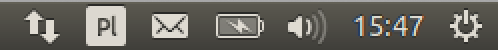
\includegraphics[width=\linewidth]{images/unity_menu_bar.png}
\end{center}

Część wskaźników widoczna jest zaraz po zainstalowaniu systemu, a cześć można dodatkowo włączyć. Niektóre aplikacja po zainstalowaniu w systemie dodają lub umożliwiają dodanie własnych wskaźników do obszaru powiadomienia. Najczęściej stosowanymi i domyślnie dostępnymi wskaźnikami w Unity są:
\begin{description}
\item[
\includegraphics{images/unity_wskaznik_klawiatura.png}]\textcolor{ubuntu_orange}{Wskaźnik klawiatury} informuje o aktualnie używanym układzie klawiatury. Klikając na niego możesz zmienić układ klawiatury.
\item[
\includegraphics{images/unity_wskaznik_siec.png}]\textcolor{ubuntu_orange}{Wskaźnik połączeń sieciowych} informuje o stanie połączenia z siecią. Kliknięcie na niego wywołuje opcje modyfikacji połączenia z internetem.
\item[
\includegraphics{images/unity_wskaznik_wiadomosci.png}]\textcolor{ubuntu_orange}{Wskaźnik wiadomości} informuje o przychodzących wiadomościach. Ten wskaźnik integruje się z komunikatorami internetowymi i zmienia kolor kiedy otrzymasz nową wiadomość. Kliknięcie na ten wskaźnik pozwala także sterować komunikatorem, np. zmienić status lub wywołać okno główne.
\item[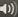
\includegraphics{images/unity_wskaznik_dzwiek.png}]\textcolor{ubuntu_orange}{Wskaźnik ustawień dźwięku} informuje o głośności wyjścia audio. Jeżeli kursor myszy znajduje się nad tym wskaźnikiem, to poruszając kółkiem myszy możesz zmienić głośność. Kliknięcie na ten wskaźnik otwiera menu ustawień dźwięku oraz menu sterownia odtwarzaczem muzyki (pozwala np. go uruchomić, zmienić utwór, wyświetlić okładkę i informacje o aktualnie odtwarzanym pliku, ustawić listę odtwarzania).
\item[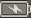
\includegraphics{images/unity_wskaznik_zasilanie.png}]\textcolor{ubuntu_orange}{Wskaźnik zasilania i poziomu akumulatora} informuje o stanie stanie naładowania akumulatora oraz o dostępnym zasilaniu (akumulator/sieć). Ten wskaźnik nie jest dostępny na komputerach pozbawionych baterii. Kliknięcie na ten wskaźnik otwiera menu zasilania.
\item[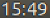
\includegraphics{images/unity_wskaznik_zegar.png}]\textcolor{ubuntu_orange}{Zegar} wyświetla aktualną datę i czas. Kliknięcie na zegar otwiera kalendarz.
\item[
\includegraphics{images/unity_wskaznik_system.png}]\textcolor{ubuntu_orange}{Wskaźnik sesji} po kliknięciu wyświetla menu systemowe, które pozwala wyłączyć/restartować komputer, wyświetlić informacje o systemie, przełączyć użytkownika lub otworzyć narzedzie konfiguracji systemu.
\end{description}

\label{unity_menu_bar}
W Unity, pasek menu aplikacji (\menu{Plik}, \menu{Edycja}, \menu{Narzędzia} itd) nie jest umieszczony w obrębie okna aplikacji, a domyślnie wyświetlany jest na pasku menu w jego lewej części. Po uruchomieniu dowolnej aplikacji pasek menu zawiera jedynie nazwę aktualnie aktywnego okna:

\begin{center}
	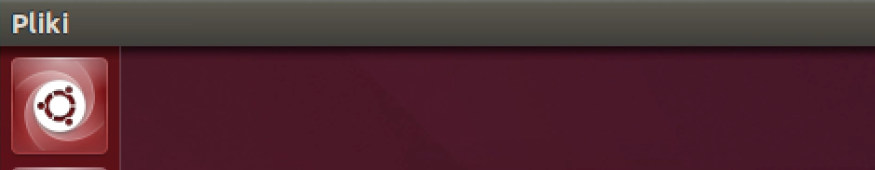
\includegraphics[width=\linewidth]{images/unity_menu_bar2.png}
\end{center}

Pasek manu jest aktywowany, gdy kursor myszy znajdzie się w obrębie panelu menu:

\begin{center}
	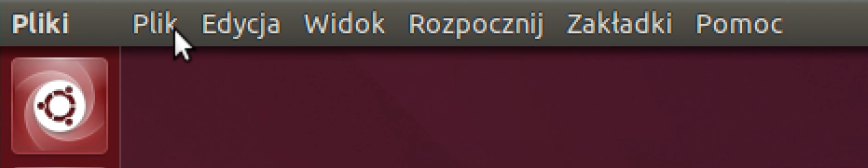
\includegraphics[width=\linewidth]{images/unity_menu_bar3.png}
\end{center}

Umieszczenie paska menu na panelu menu ma swoje plusy w przypadku urządzeń z ekranem ograniczonym niską rozdzielczością. Tak zwane \textcolor{ubuntu_orange}{Global Menu} Pozwala lepiej wykorzystać dostępne miejsce w pionie.